\documentclass[a4paper,11pt,oneside]{report}

%%%%%%%%%%%%%%%%%%%%%
% Encodage et langues
\usepackage[numbers]{natbib}
\usepackage[main=french,english]{babel}
\usepackage{fontspec}
\usepackage{xeCJK}
\setCJKmainfont{FandolSong}
\setCJKsansfont{FandolHei}
\setCJKmonofont{FandolFang}

%%%%%%%%%%%%%%%%%%%%%
% Liens et métadonnées
\usepackage[colorlinks=false, breaklinks, pdfborder={0 0 0}]{hyperref}

%%%%%%%%%%%%%%%%%%%%%
% Mise en page et utilitaires
\usepackage{float}
\usepackage{amsmath}
\usepackage{amssymb}
\usepackage{geometry}
\geometry{a4paper, margin=2.5cm, headheight=17pt}
\usepackage{graphicx}
\usepackage{caption}
\usepackage{booktabs}
\usepackage{longtable}
\usepackage{listings}
\usepackage{xcolor}
\usepackage{enumitem}
\usepackage{fancyhdr}
\usepackage{setspace}

% Rendre les listes moins "visuelles" et plus compactes (réduit la fatigue à la lecture)
\setlist[itemize]{label=\textendash, leftmargin=*, nosep}

\lstset{
	    basicstyle=\ttfamily\footnotesize,
	    breaklines=true,
	    frame=single,
    backgroundcolor=\color{gray!5},
    literate={é}{{\'e}}1 {è}{{\`e}}1 {à}{{\`a}}1 {ç}{{\c{c}}}1 {œ}{{\oe}}1 {ù}{{\`u}}1 {É}{{\'E}}1 {È}{{\`E}}1 {À}{{\`A}}1 {Ç}{{\c{C}}}1 {Œ}{{\OE}}1 {Ê}{{\^E}}1 {ê}{{\^e}}1 {î}{{\^i}}1 {ô}{{\^o}}1 {û}{{\^u}}1
}

\lstdefinelanguage{pseudo}{
    morekeywords={for,foreach,while,if,else,return},
    sensitive=false
}

\newcommand{\bigO}[1]{\ensuremath{\mathop{}\mathopen{}O\mathopen{}\left(#1\right)}}
\newcommand{\smallO}[1]{\ensuremath{\mathop{}\mathopen{}o\mathopen{}\left(#1\right)}}

\captionsetup[figure]{font=footnotesize, justification=justified, singlelinecheck=false, position=bottom}
\captionsetup[table]{font=footnotesize, justification=justified, singlelinecheck=false, position=top}
\urlstyle{same}
\emergencystretch=1em

\setcounter{tocdepth}{3}
\setcounter{secnumdepth}{3}
\setstretch{1.2}
\setlength{\parindent}{2em}
\setlength{\parskip}{0pt}
\renewcommand{\contentsname}{Sommaire}
\renewcommand{\bibname}{Références}

\newcommand{\reporttype}{Rapport de projet}
\newcommand{\reporttitletext}{MLP et moteur d'autodiff appliqués à MNIST}
\newcommand{\reportshorttitle}{MLP et moteur d'autodiff}
\newcommand{\reportauthors}{Jianye Shi, Hao Qian, Xiang Bian, Abdennour Boulmis}
\newcommand{\reportadvisor}{Aurélien Delval}
\newcommand{\reportprogram}{Master 1 CHPS -- UVSQ}
\newcommand{\reportyear}{Année universitaire 2025--2026}
\newcommand{\reportdate}{4 avril 2026}

%%%%%%%%%%%%%%%%%%%%%
% En-têtes et pieds de page
\fancyhf{}
\fancyhead[L]{\textit{\reportshorttitle}}
\fancyhead[R]{\nouppercase{\leftmark}}
\fancyfoot[C]{\thepage}
\renewcommand{\headrulewidth}{0.4pt}
\renewcommand{\footrulewidth}{0pt}
\setlength{\headheight}{17pt}
\renewcommand{\chaptermark}[1]{\markboth{\thechapter.\ #1}{}}
\fancypagestyle{plain}{
  \fancyhf{}
  \fancyfoot[C]{\thepage}
  \renewcommand{\headrulewidth}{0pt}
  \renewcommand{\footrulewidth}{0pt}
}

\begin{document}

\hypersetup{pageanchor=false}
\pagenumbering{gobble}
\begin{titlepage}
  \centering
  \vspace*{0.9cm}
  
\includegraphics[width=0.38\textwidth]{Images/Logo_UVSQ.jpg}\par
  \vspace{1.0cm}
  {\Large \reportprogram\par}
  \vspace{0.45cm}
  {\large \reportyear\par}
  \vspace{2.8cm}
  {\large \reporttype\par}
  \vspace{0.6cm}
  {\huge\bfseries \reporttitletext\par}
  \vspace{3.2cm}
  \begin{flushleft}
    \textbf{Auteurs :}\par
    \reportauthors\par
    \vspace{0.75cm}
    \textbf{Encadrant :}\par
    \reportadvisor\par
  \end{flushleft}
  \vfill
  {\large \reportdate\par}
\end{titlepage}

\clearpage
\hypersetup{pageanchor=true}
\pagenumbering{roman}
\setcounter{page}{1}
\chapter*{Résumé}
\addcontentsline{toc}{chapter}{Résumé}
Ce rapport présente les travaux du second semestre, prolongeant un premier prototype fondé sur un MLP, un moteur d'autodifférentiation en C++ et des optimisations matricielles validées sur MNIST. L'objectif du semestre 2 est d'élargir ce socle vers un pipeline d'entraînement plus réaliste et plus instrumenté. Les principales extensions portent sur l'introduction d'une architecture CNN configurable, la prise en charge du jeu de données Tiny-ImageNet, l'ajout d'un mode distribué par synchronisation de gradients sous MPI, ainsi que la génération d'artefacts d'exécution pour l'analyse de performance et la reproductibilité. Les développements réalisés montrent que le projet ne se limite plus à un démonstrateur pédagogique centré sur MLP/MNIST, mais constitue désormais une base expérimentale plus large pour l'étude de charges de travail visuelles, de mécanismes de synchronisation et de backends de calcul alternatifs. Le rapport précise enfin le statut actuel des fonctionnalités stabilisées, en qualification ou encore exploratoires.

\bigskip
\noindent\textbf{Mots-clés :} autodifférentiation, CNN, Tiny-ImageNet, MPI, C++, reproductibilité, profiling, optimisation

\clearpage
\tableofcontents
\clearpage
\pagenumbering{arabic}
\setcounter{page}{1}
\pagestyle{fancy}

\chapter{Introduction générale}
\section{Rappel du semestre 1}
Le premier semestre du projet a permis d'établir un socle fonctionnel autour d'un Perceptron Multicouche (MLP) entraîné sur MNIST \cite{lecun1998}. Cette première étape a conduit à l'implémentation d'un moteur d'autodifférentiation en mode inverse, d'une représentation explicite du graphe de calcul, d'un noyau matriciel optimisable et d'une boucle d'entraînement complète en C++. Elle a également permis de valider la convergence du modèle sur une tâche de classification standard, puis de mettre en évidence l'importance des optimisations bas niveau, notamment via BLAS et OpenMP, sur le temps d'exécution.

\section{Motivations et objectifs du semestre 2}
Si cette première version constituait une base pédagogique solide, elle restait limitée à un cadre relativement simple : un modèle de type MLP, un jeu de données de petite taille et un scénario d'exécution essentiellement monoprocessus. Le second semestre vise donc à faire évoluer le projet vers un environnement plus proche d'un pipeline d'entraînement réaliste. Les objectifs principaux sont l'extension vers des architectures convolutionnelles configurables, l'intégration d'un jeu de données d'images plus exigeant avec Tiny-ImageNet, l'étude de la synchronisation de gradients dans un cadre distribué sous MPI, ainsi que la mise en place d'outils d'instrumentation et d'artefacts permettant une analyse plus rigoureuse des performances et de la reproductibilité.

Dans cette perspective, le semestre 2 ne consiste pas à réécrire le projet initial, mais à prolonger l'infrastructure développée au semestre 1 pour en faire une base expérimentale plus large. Il s'agit à la fois d'augmenter la complexité des charges de travail traitées, de renforcer la dimension système du projet et de clarifier le statut des différentes fonctionnalités introduites, qu'elles soient stabilisées, en cours de qualification ou encore exploratoires.

\section{Organisation du rapport}
Le rapport s'articule autour de cinq axes :
\begin{enumerate}[label=\textbf{\arabic*.}, leftmargin=*, nosep]
  \item \textbf{Fondements théoriques et périmètre} : rappel du cadre d'étude et des notions mobilisées par le projet.
  \item \textbf{Conception et réalisation} : présentation des extensions logicielles introduites au second semestre.
  \item \textbf{Protocole expérimental et résultats} : description des configurations d'essai, des métriques retenues et des observations obtenues.
  \item \textbf{Organisation du projet} : synthèse de la conduite du développement et de la répartition des contributions.
  \item \textbf{Conclusion et perspectives} : bilan du semestre 2, limites actuelles et pistes d'évolution.
\end{enumerate}
Des annexes techniques et un glossaire complètent enfin le document.

\chapter{GEMM矩阵乘法的优化}

本章系统阐述矩阵乘法（GEMM，\textit{General Matrix Multiply}）的逐步优化历程。
矩阵乘法是神经网络训练中最核心的计算操作，其性能直接决定了训练速度的上限。
优化路径从分析OpenBLAS的多线程行为出发，经由OpenMP手动分块与打包实验，
最终抵达具有自定义SIMD微内核的GotoBLAS架构，并在真实神经网络负载下与OpenBLAS进行全面对比。

\section{实验环境}

\subsection{硬件平台}

\begin{table}[H]
\centering
\caption{GEMM实验硬件配置}
\label{tab:gemm_hardware}
\begin{tabular}{p{0.28\textwidth}p{0.62\textwidth}}
\toprule
\textbf{组件} & \textbf{规格} \\
\midrule
处理器 & AMD Ryzen 9 8940HX，x86\_64架构 \\
物理核心/逻辑线程 & 16物理核心，32逻辑线程（每核2线程，SMT）\\
实验限制 & 通过 \texttt{taskset -c 0-7} 限制到8个CPU，并通过 \texttt{lscpu -e=CPU,CORE,SOCKET,NODE} 验证其物理核心映射 \\
缓存层次 & L1d 32 KiB/核，L2 1 MiB/核，L3 64 MiB（共享）\\
运行频率 & 锁定在4.0 GHz（禁用Turbo Boost）\\
内存 & 30 GiB \\
\bottomrule
\end{tabular}
\end{table}

\subsection{软件环境}

\begin{table}[H]
\centering
\caption{GEMM实验软件配置}
\label{tab:gemm_software}
\begin{tabular}{p{0.28\textwidth}p{0.62\textwidth}}
\toprule
\textbf{组件} & \textbf{版本/详情} \\
\midrule
操作系统 & Fedora Linux 42 \\
编译器 & GCC 15.2.1，编译选项 \texttt{-O3 -march=native} \\
BLAS库 & OpenBLAS（系统版本）\\
并行模型 & OpenMP 5.0 \\
向量指令集 & AVX2 / AVX-512（通过 \texttt{-march=native} 自动启用）\\
\bottomrule
\end{tabular}
\end{table}

\subsection{测量协议}\label{subsec:gemm_protocol}

为确保测量结果的可靠性，我们采用如下严格协议：
\begin{itemize}
    \item \textbf{预热（Warm-up）}：每组测试前执行5次预热迭代，以稳定指令缓存和数据缓存状态；
    \item \textbf{计时}：程序内部循环2000次，使用 \texttt{std::chrono::high\_resolution\_clock} 精确计时；
    \item \textbf{硬件计数器}：通过 \texttt{perf stat -r 3} 外部重复3次，采集指令数（Instructions）、
          周期数（Cycles）、上下文切换（Context Switches）、CPU迁移（CPU Migrations）及缓存缺失（Cache Misses）；
    \item \textbf{环境隔离}：关键批次之间重启系统，清空页缓存（\texttt{drop\_caches}），
          通过 \texttt{cpupower} 锁定CPU频率，以减少系统状态异质性。
          预热是稳定执行路径的主要机制；重启和清空页缓存仅用于降低系统整体状态带来的跨批次干扰。
\end{itemize}

需特别指出：\texttt{perf} 的 \texttt{:u}（用户态）修饰符会排除在内核态发生的上下文切换，
因此本实验一律使用无修饰符的 \texttt{context-switches}，以捕获完整的内核调度事件。
此外，AMD uncore L3事件以system-wide方式采集，短窗口下易受后台进程污染，因此本文不将其用于定量比较，
而采用per-task的 \texttt{cache-misses} 与 \texttt{cache-references} 作为聚合性内存压力指标；
\texttt{cache-misses} 本身是聚合性事件，本文仅用于不同配置之间的相对比较，不用于精确区分L1/L2/L3层级来源。

\paragraph{CPU余量与实验隔离。}
本报告并不追求占满机器上所有逻辑线程，而是将GEMM实验限制在一个可控的CPU核心预算内。
这样做可以为操作系统、OpenMP运行时、\texttt{perf}采集以及后台服务保留一定CPU余量，
减少线程迁移、中断和非受控资源竞争。
该设置也使后文能够区分两类配置：一类是限制在已验证物理核心预算内的推荐配置，
另一类是16线程SMT/超线程压力测试配置，用于分析过度并行带来的调度和同步开销。

\section{OpenBLAS多线程分析：超线程的代价}\label{sec:gemm_smt}

在进行底层优化之前，我们首先系统研究了OpenBLAS的GEMM与OpenMP的GEMM基础并行实现（未进行除omp外任何优化）在1至16线程下的扩展性，
以理解超线程（SMT）对GEMM计算任务的性能的具体影响。

\subsection{初步观察}

图~\ref{fig:blas1_scaling}展示了未绑定CPU核心时两种实现的线程扩展性。

\begin{figure}[H]
    \centering
    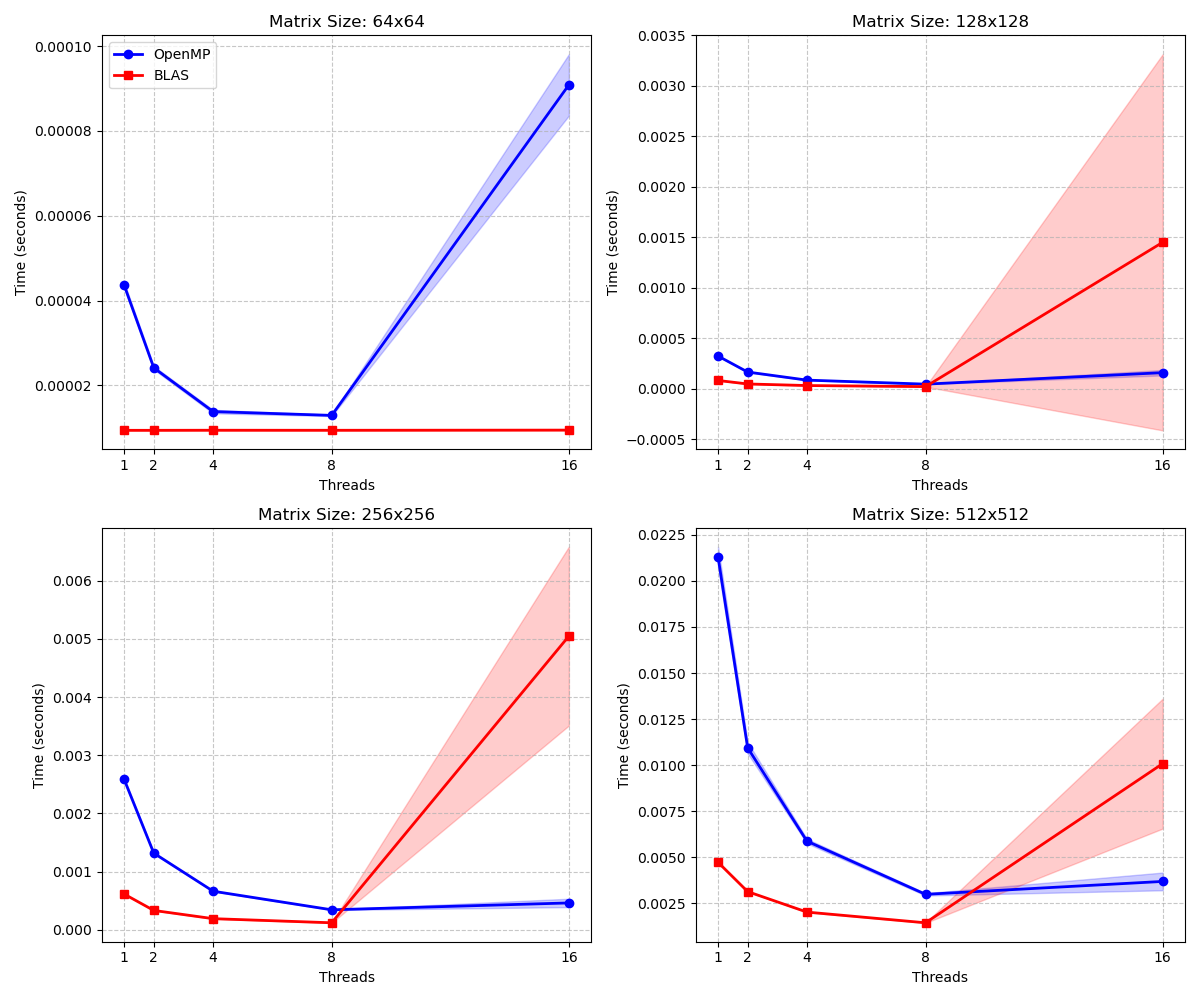
\includegraphics[width=0.90\textwidth]{../output/ExperienceGEMM/BLAS1/scaling_plot_advanced.png}
    \caption{初始实验（BLAS1）：线程数对BLAS与OMP性能的影响（未绑定CPU核心）。
             纵轴为执行时间（$\mu$s），横轴为线程数，分四个矩阵尺寸展示。}
    \label{fig:blas1_scaling}
\end{figure}

两个关键现象立即显现：

\textbf{现象一：BLAS对64×64矩阵保持单线程行为。}
64×64矩阵的计算量仅约524K FLOP，未达到OpenBLAS内部的并行化触发阈值。
因此，无论配置多少线程，BLAS始终以单线程执行，时间稳定在约9.4~$\mu$s。
基础OpenMP手动并行在8线程下可将时间降至4.4~$\mu$s；该结果说明基础OpenMP对极小矩阵存在短路径优势，
不能据此说明OpenBLAS多线程策略有问题。

\textbf{现象二：16线程（超线程）引发两类性质不同的性能退化。}
在16线程配置下，两类异常需要区分。
OMP在64×64上执行时间从8.97~$\mu$s增至73.00~$\mu$s（退化\textbf{8.1倍}），
说明极小矩阵对过度并行非常敏感；但由于该实现是基础OpenMP GEMM，
该现象可能同时受到barrier开销、调度粒度、false sharing或手写并行结构等因素的影响，
因此本文不将其作为OpenBLAS内部行为的直接证据。
相比之下，OpenBLAS在128×128至512×512上出现的指令数暴增（128×128时达到8线程的\textbf{252倍}）和方差极大，
才是后续16线程诊断实验的主要对象。

\subsection{16线程异常的解释}

以下诊断主要针对OpenBLAS在128×128及以上矩阵中的16线程异常，而不是对OMP 64×64退化的唯一归因。OpenBLAS的高性能内核（GotoBLAS风格实现）通常已能充分占用物理核心的FMA单元、SIMD寄存器、L1/L2缓存带宽及load/store端口；SMT不增加新的物理执行单元，两个逻辑核心共享同一套物理资源，因此在计算密集型负载下，16线程在8个物理核心上难以带来额外收益，且会引入竞争成本。小矩阵场景中，计算量极小，线程在barrier处的自旋等待时间占比极高，同步和调度的相对开销被进一步放大。

附录~\ref{app:smt_diagnosis}中的三组对照实验提供了量化支持，但其诊断对象不同，需分别解读。
需指出，本文中IPC不用于直接排序OMP与BLAS的优劣，而是结合执行时间、指令数和调度事件作为异常诊断信号（OMP的高IPC部分源于轻量同步指令占比较高，而非计算效率更高）。
矩阵规模效应分析（实验A）以OMP为测量对象，显示OMP 128×128的每操作指令数（Instr/Op）为0.587，而1024×1024仅为0.128，差距4.5倍。该实验说明小矩阵下固定同步开销占比被放大的通用现象，可为分析OpenBLAS同类行为提供数学参考，但不构成对OpenBLAS内部机制的直接测量证明。
如图~\ref{fig:cs_comparison}所示，BLAS1扩展性实验中OMP 64×64的16线程配置出现约89{,}617次context switches；该数字反映基础OpenMP小矩阵的过度并行风险，可能包含false sharing、barrier和任务粒度等实现因素，不应直接用于解释OpenBLAS的内部行为，在此仅作旁证。
诊断OpenBLAS 128×128异常的核心证据来自单独设计的亲和性对照实验（实验B，OpenBLAS、16线程、128×128、5000次迭代）：绑定核心后指令数从13.45\,B降至4.05\,B（$-69.9\%$），context switches从2{,}013降至14（$-99.3\%$），缓存缺失标准差改善约22倍。这些结果强支持调度/迁移与同步等待开销是当前最一致的主导解释，但尚未完全排除内存带宽竞争等其他因素的贡献。

补充窗口稳定性分析（实验C）表明，16线程配置下500次迭代的缓存缺失变异系数高达30.3\%，2000次迭代时降至1.4\%，说明该配置的测量稳定性对采样窗口长度较为敏感，标准2000次窗口在本实验条件下已提供可信的统计基础。

\begin{figure}[H]
    \centering
    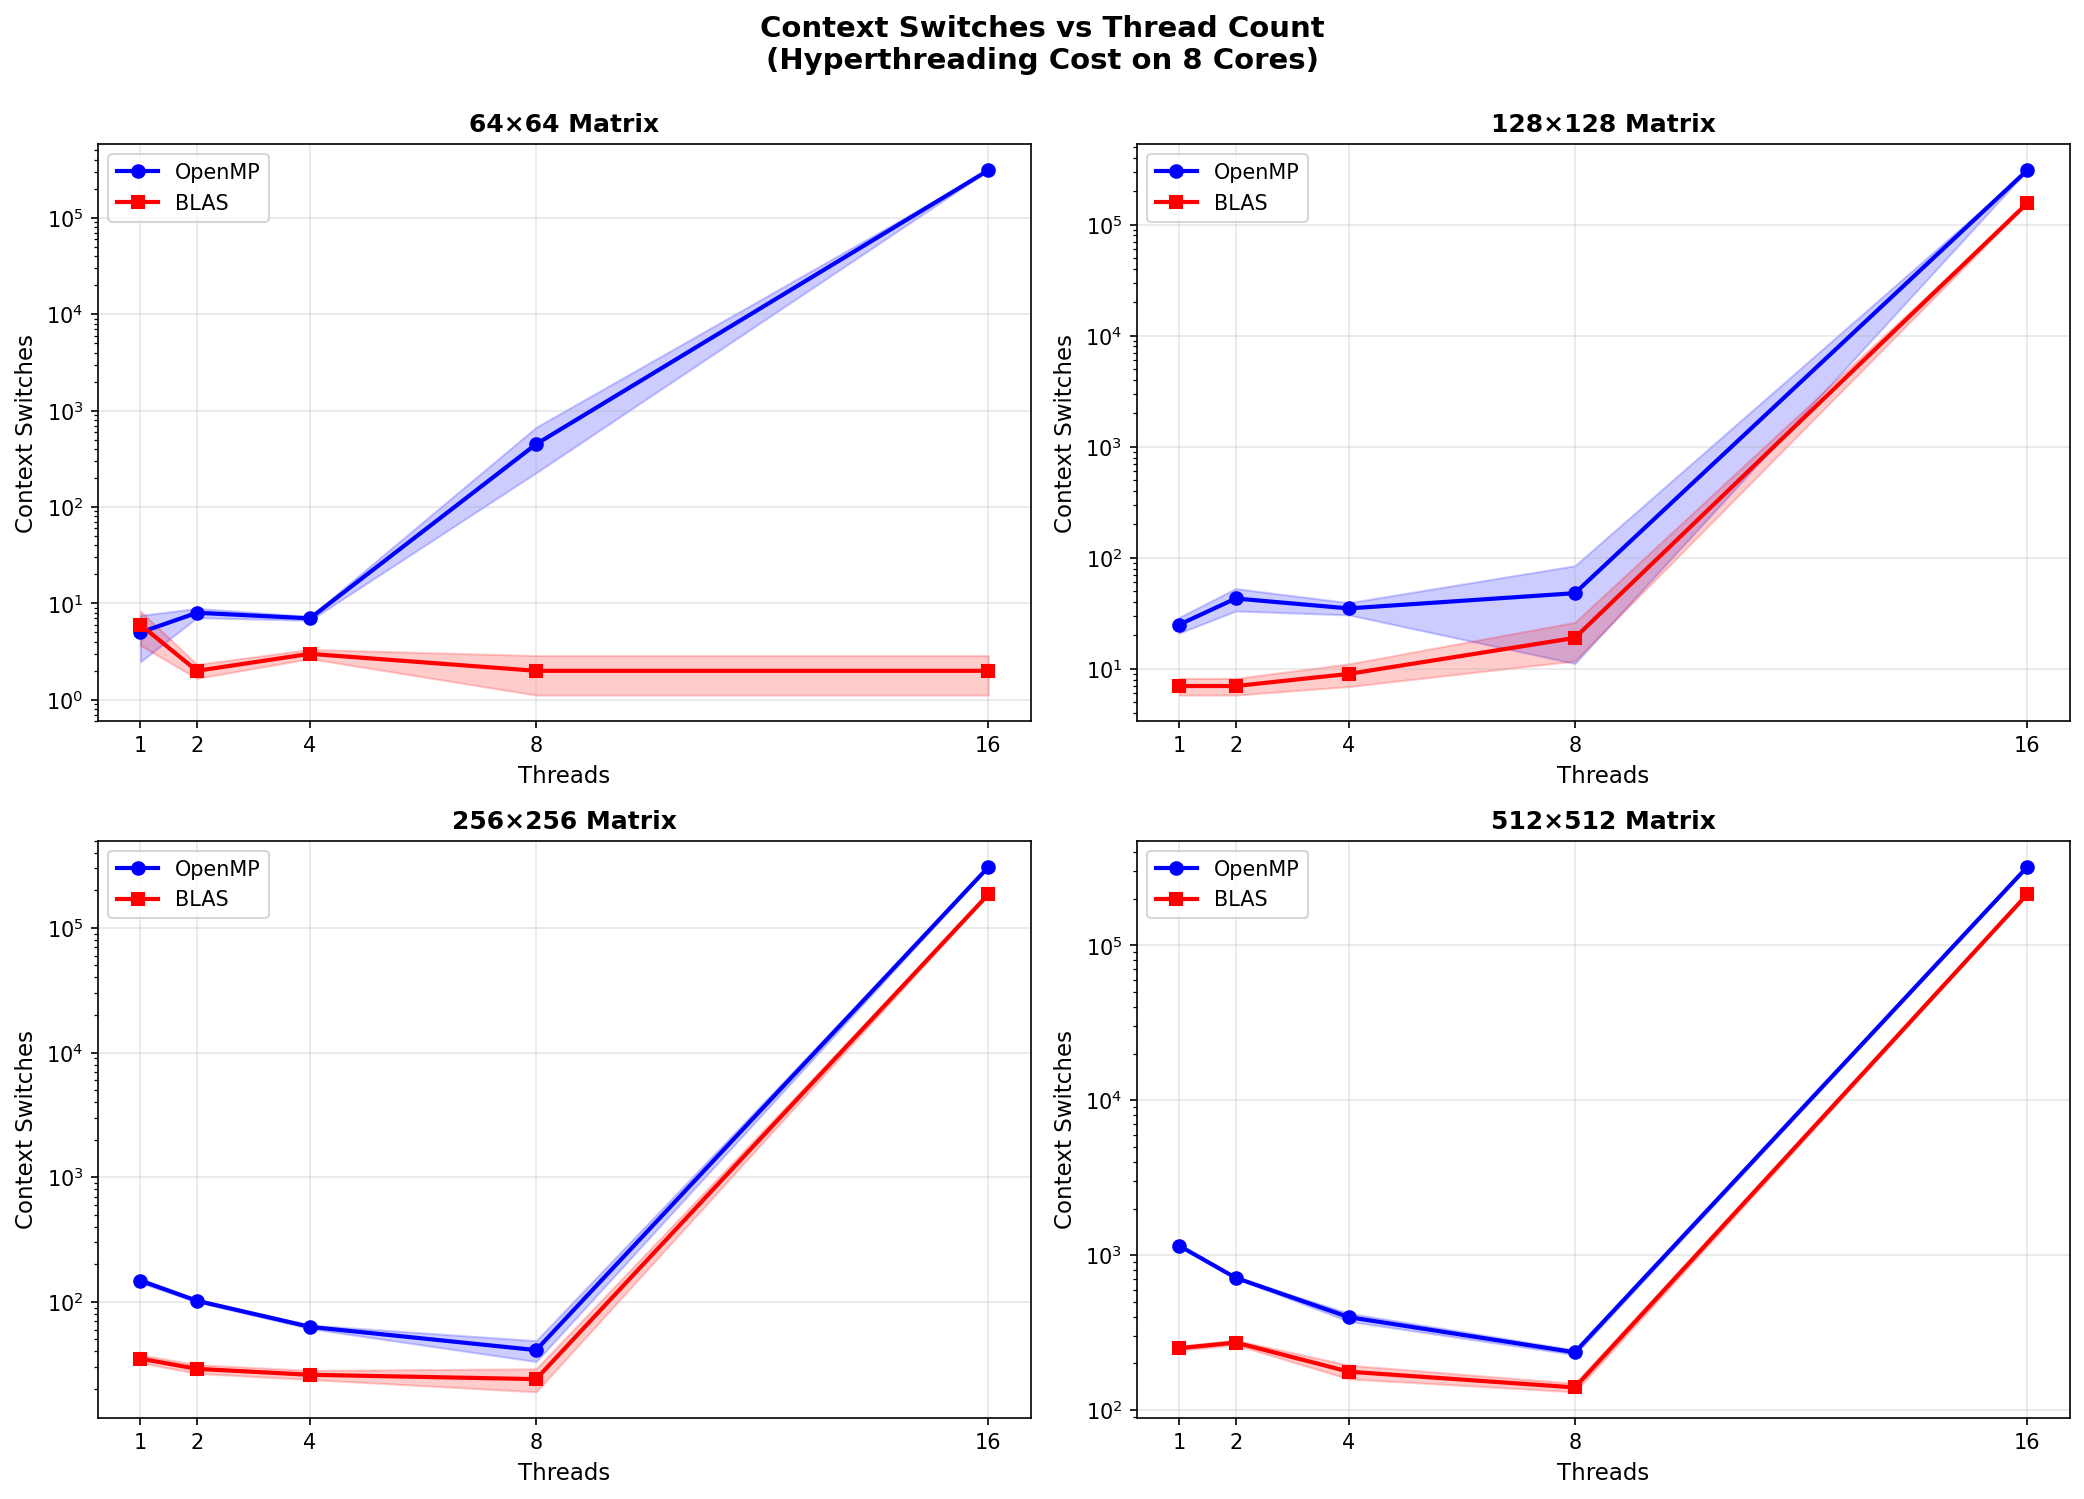
\includegraphics[width=0.90\textwidth]{../output/ExperienceGEMM/BLAS1/context_switches_vs_threads.png}
    \caption{BLAS1扩展性实验中的上下文切换次数（未绑定核心）。
             OMP 64×64的极端值说明极小矩阵过度并行的风险；
             该图本身不直接反映OpenBLAS 128×128的内部自旋等待机制，
             后者需结合亲和性对照实验（实验B）解读。}
    \label{fig:cs_comparison}
\end{figure}

\subsection{结论：限制到物理核心，强制绑定}

综合上述结果，16线程配置在两类实现上均不适合作为推荐配置。
对于OpenBLAS而言，亲和性对照实验表明绑定线程可显著降低调度事件和同步等待相关指令，支持将线程数控制在物理核心预算以内。
对于基础OpenMP而言，OMP 64×64的极端退化说明小矩阵过度并行风险较高，其成因可能涉及多种实现因素。

\textbf{因此，后续所有实验均限制在1至8个物理线程，并强制启用 \texttt{OMP\_PROC\_BIND=true} 与 \texttt{OMP\_PLACES=cores}。}
这一选择同时为系统和测量工具保留CPU余量，而不是占满所有逻辑线程。

图~\ref{fig:blas2_scaling}展示了施加CPU亲和性约束后的性能对比——各实现均趋于稳定，
BLAS在8线程下成为各矩阵尺寸的最优配置。

\begin{figure}[H]
    \centering
    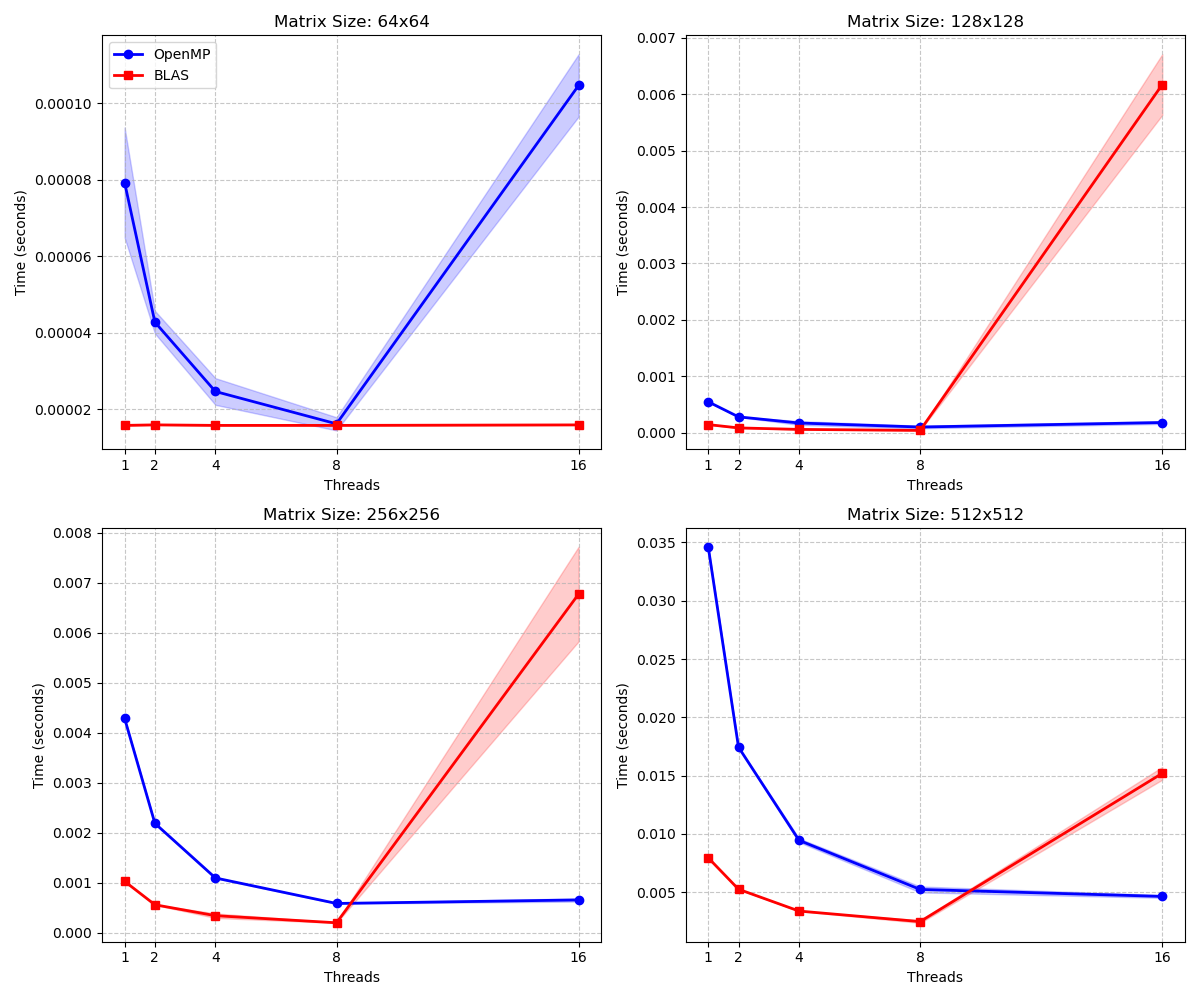
\includegraphics[width=0.90\textwidth]{../output/ExperienceGEMM/BLAS2/scaling_plot_advanced.png}
    \caption{施加CPU亲和性约束后（BLAS2）的线程扩展性对比。
             BLAS在8线程下为所有矩阵尺寸的最优选择。}
    \label{fig:blas2_scaling}
\end{figure}

\begin{table}[H]
\centering
\caption{施加亲和性约束后各矩阵尺寸的最优配置（OpenBLAS）}
\label{tab:blas_optimal}
\begin{tabular}{lrrl}
\toprule
\textbf{矩阵尺寸} & \textbf{最优配置} & \textbf{性能 ($\mu$s)} & \textbf{相比单线程加速} \\
\midrule
64×64   & BLAS 单线程 & 9.42    & ---          \\
128×128 & BLAS 8线程  & 24.29   & $3.5\times$  \\
256×256 & BLAS 8线程  & 123.75  & $5.0\times$  \\
512×512 & BLAS 8线程  & 1428.53 & $3.3\times$  \\
\bottomrule
\end{tabular}
\end{table}

\section{OpenMP分块与打包技术}

在理解OpenBLAS行为的基础上，我们转向自主实现的OpenMP GEMM，
系统探索\textbf{分块（Blocking）}和\textbf{数据打包（Packing）}技术对性能的影响。
这一系列实验旨在通过实践理解GotoBLAS架构的核心思想。

\subsection{基础分块：\texttt{omp\_blocked}}

朴素的$ikj$排序GEMM已具备较好的内层循环访存局部性，
但当矩阵规模增大时，B矩阵的列访问仍会引起频繁的缓存缺失。
\textbf{分块GEMM}将大矩阵分解为小tile（大小由 \texttt{MATMUL\_BLOCK\_SIZE} 控制），
确保tile在计算过程中保留在缓存中，减少数据的重复加载。

实验扫描了tile大小 $\in \{32, 48, 64\}$，测试矩阵尺寸64至512、线程数1至8。
结果表明：对于256×256至512×512的矩阵，tile=64在多线程下表现最优；
小矩阵（64×64）对分块大小不敏感，因为整个矩阵已适配L1缓存。

\subsection{带打包的分块：\texttt{omp\_blocked\_packed}与\texttt{omp\_blocked\_packab}}

即使经过分块，多线程间仍共享同一内存视图，导致\textbf{伪共享}（False Sharing）
和跨核心TLB压力。打包技术通过将即将使用的数据块以\textbf{连续格式}
复制到线程私有缓冲区来解决此问题：

\textbf{\texttt{omp\_blocked\_packed}}：在每个K维度面板（Panel）开始前，
将B矩阵的对应列打包至连续私有缓冲区，使B面板的读取成为步长为1的顺序访问，
显著改善硬件预取器的效率。

\textbf{\texttt{omp\_blocked\_packab}}：在前者基础上，同时对A矩阵的行面板打包，
并采用分阶段扫描策略单独优化三个打包维度的参数：
\texttt{PACK\_M} $\in \{32, 48, 64, 96, 128\}$、
\texttt{PACK\_N} $\in \{32, 48, 64, 96, 128\}$、
\texttt{PACK\_K} $\in \{16, 24, 32, 48, 64, 96\}$。
分阶段扫描（每次只改变一个轴）使得性能变化可明确归因于具体参数。

\subsection{关键发现}

打包技术在大矩阵下显著改善了多线程性能，
尤其是PACK\_K约为32至64时，L2缓存利用率最高。
然而，与OpenBLAS相比，即使经过完整的A+B双打包，性能差距仍然显著。

\textbf{根本原因}在于：我们的分块实现缺乏针对SIMD寄存器优化的微内核，
无法充分利用AVX2的FMA（Fused Multiply-Add）指令实现峰值浮点吞吐。
这直接引出了GotoBLAS的设计思想，即将SIMD微内核与分块打包结合为一体。

\section{GotoBLAS架构}\label{sec:gotoblas_arch}

GotoBLAS（由Kazushige Goto开创，现由OpenBLAS继承）的核心创新在于
将GEMM分解为\textbf{层次化缓存感知分块}，并在最内层使用\textbf{手工汇编SIMD微内核}，
将L1/L2缓存复用最大化的同时保持寄存器级别的计算密度。

\subsection{三层分块模型}

GotoBLAS将 $C = A \cdot B$（规模 $M \times K \times N$）分解为三层嵌套循环，
每层对应一个缓存层级：

\begin{enumerate}
    \item \textbf{外层（$N_c$维度）}：沿N维度以$N_c$为步长，将B的面板（$K \times N_c$）装入LLC（L3缓存）；
    \item \textbf{中层（$K_c$维度）}：沿K维度以$K_c$为步长，将打包后的B面板（$K_c \times N_c$）装入L2缓存；
    \item \textbf{内层（$M_c$维度）}：沿M维度以$M_c$为步长，将打包后的A面板（$M_c \times K_c$）装入L1缓存；
    \item \textbf{微内核（$M_r \times N_r$寄存器tile）}：最内层操作，在SIMD寄存器中积累$M_r \times N_r$的C块。
\end{enumerate}

\begin{lstlisting}[language=pseudo, caption={GotoBLAS三层分块结构伪代码}]
for nc = 0 to N step Nc:
    Pack B[0:K, nc:nc+Nc] -> B_panel (in L3/L2)
    for kc = 0 to K step Kc:
        for mc = 0 to M step Mc:
            Pack A[mc:mc+Mc, kc:kc+Kc] -> A_panel (in L1)
            for nr = 0 to Nc step Nr:
                for mr = 0 to Mc step Mr:
                    // Mr x Nr SIMD微内核：FMA寄存器tile累加
                    C[mr..mr+Mr, nr..nr+Nr] += MicroKernel(A_panel, B_panel)
\end{lstlisting}

缓存块参数通过以下原则推导：
$M_c \times K_c \times 8$字节的A面板目标适配L1缓存（32~KiB/核）；
$K_c \times N_c \times 8$字节的B面板目标适配L2缓存（1~MiB/核）。
本实现的默认参数为$K_c=384$，$M_c$有效行数=64（倍率8，基于$M_r=8$），$N_c=448$，
这些参数通过实验调优进一步验证（见第~\ref{sec:avx2_tuning}节）。

\subsection{微内核设计}\label{subsec:microkernel}

微内核是性能的核心。以\textbf{AVX2 8×8微内核}（$M_r=8, N_r=8$）为例：
AVX2的YMM寄存器宽度为256位，可同时处理4个双精度浮点数。
一个8×8的C寄存器tile需要 $M_r \times (N_r/4) = 8 \times 2 = 16$个YMM寄存器，
恰好对应AVX2提供的16个可用YMM寄存器，实现\textbf{满寄存器利用（Full Register Utilization）}。

类似地，\textbf{4×16微内核}（$M_r=4, N_r=16$）同样需要 $4 \times 4 = 16$个寄存器，
通过更宽的N方向向量化降低边界处理（Edge Case）开销，在N维度较大时有优势。

本项目实现的AVX2微内核列举如下：

\begin{table}[H]
\centering
\caption{已实现的GotoBLAS AVX2微内核}
\label{tab:kernels_avx2}
\begin{tabular}{lrrl}
\toprule
\textbf{内核名称} & $M_r$ & $N_r$ & \textbf{主要特点} \\
\midrule
\texttt{avx2\_8x8}  & 8  & 8  & 16寄存器满载，通用性强 \\
\texttt{avx2\_4x16} & 4  & 16 & 宽N方向，适合$N$较大形状 \\
\texttt{avx2\_12x8} & 12 & 8  & 高$M$覆盖率 \\
\texttt{avx2\_13x8} & 13 & 8  & 扩展$M$覆盖 \\
\texttt{avx2\_5x16} & 5  & 16 & 中等$M$，宽N \\
\texttt{avx2\_6x16} & 6  & 16 & 中等$M$，宽N \\
\bottomrule
\end{tabular}
\end{table}

AVX-512微内核（如\texttt{avx512\_8x32}）将在第~\ref{sec:avx512_brief}节简介；
完整推理见附录~\ref{app:avx512_tuning}。

\section{GotoBLAS单线程调优：AVX2微内核筛选}\label{sec:avx2_tuning}

理论参数仅为起点，实际最优参数因工作负载形状和缓存行为而异，
必须通过系统实验搜索确定。
本节描述针对神经网络GEMM形状的单线程调优方法论及主要结果。

\subsection{测试工作负载}

参照项目MLP和CNN的实际层形状，定义了4个代表性工作负载族（Workload Family）：

\begin{table}[H]
\centering
\caption{单线程调优使用的代表性工作负载（batch=32）}
\label{tab:tuning_workloads}
\begin{tabular}{llrrr}
\toprule
\textbf{工作负载族} & \textbf{来源层} & $M$ & $K$ & $N$ \\
\midrule
fc\_forward\_mainstream & MLP FC1（hidden=128） & 32 & 784 & 128 \\
fc\_head\_small\_n      & MLP FC2（output）      & 32 & 128 & 10  \\
conv\_dx\_skinny\_k     & CNN Conv2 backward     & 3200 & 16 & 150 \\
fc\_wide\_output        & MLP FC1（hidden=256）  & 32 & 784 & 256 \\
\bottomrule
\end{tabular}
\end{table}

\subsection{两轮搜索策略}

\textbf{第一轮（全局候选筛选）}：
对所有6种AVX2内核，在各工作负载上扫描多个$(M_c, N_c, K_c)$组合（共272个候选）。
每候选运行1000次取中位时间，并辅以5次\texttt{perf stat}采样记录硬件计数器。
采用分阶段扫描策略：先固定$M_c, N_c$扫$K_c$，再固定最优$K_c$扫$M_c$，最后精扫$N_c$，
使得性能变化可明确归因于单一参数轴。

\textbf{第二轮（局部精细化）}：
保留第一轮中在主流FC形状上表现最佳的5个\texttt{KernelShape/Kc}组合：
\texttt{8x8/Kc=288}、\texttt{8x8/Kc=384}、\texttt{4x16/Kc=192}、
\texttt{4x16/Kc=256}、\texttt{4x16/Kc=320}，
在其最优区域周围加密$M_c, N_c$搜索网格（每行约75个组合），进一步精确定位最优参数。

\subsection{调优结果}

图~\ref{fig:avx2_heatmap}展示了第一轮搜索结果的热图，
颜色越深（绿色）代表与最优自定义实现的差距越小。

\begin{figure}[H]
    \centering
    
\includegraphics[width=0.88\textwidth]{../output/ExperienceGEMM/GotoBLASBlocked/summary/plots/relative_to_best_custom_heatmap.png}
    \caption{AVX2单线程候选热图：各内核形状在代表性工作负载上相对于最佳自定义实现的GFLOPS比值（\%）。}
    \label{fig:avx2_heatmap}
\end{figure}

主要结论汇总于下表：

\begin{table}[H]
\centering
\caption{AVX2单线程调优：各工作负载族的最佳配置及与OpenBLAS单线程的对比}
\label{tab:avx2_tuning_results}
\begin{tabular}{p{0.24\textwidth}lrrrrrr}
\toprule
\textbf{工作负载族} & \textbf{最优内核} & $M_c$ & $N_c$ & $K_c$ &
\textbf{自定义} & \textbf{OpenBLAS} & \textbf{差距} \\
 & & & & & \textbf{($\mu$s)} & \textbf{($\mu$s)} & \\
\midrule
fc\_forward (b32) & 4x16 & 128 & 576 & 320 & 72.5  & 60.2 & $-17\%$ \\
fc\_forward (b64) & 4x16 & 192 & 512 & 256 & 132.6 & 110.1 & $-17\%$ \\
fc\_head (b32)    & 4x16 & --  & --  & --  & 4.76  & 1.14 & $-76\%$ \\
conv\_dx (b32)    & 8x8  & 160 & 640 & 288 & 744.3 & 647.3 & $-13\%$ \\
fc\_wide (b32)    & 4x16 & 128 & 768 & 256 & 136.5 & 122.2 & $-10\%$ \\
\bottomrule
\end{tabular}
\end{table}

结果揭示了两类性能差距：

\textbf{主流形状（$N \geq 64$）}：与OpenBLAS的差距在10至24\%之间，
反映了我们微内核实现与高度优化的OpenBLAS汇编之间的性能差距，
以及OpenBLAS针对特定形状的更精细适配（如padding和prefetch策略）。

\textbf{小N形状（$N < 32$，如fc\_head）}：差距高达66至78\%。
极小的$N$无法形成有效的$N_r$寄存器tile，导致大量边界处理开销。
OpenBLAS对退化形状有专用代码路径，而本实现尚未针对此类形状优化。

\subsection{最终AVX2配置与AVX-512简介}\label{sec:avx512_brief}

综合单线程调优结果，选定如下固定配置用于多线程实验：
\[
\texttt{avx2\_8x8},\quad K_c = 384,\quad M_c = 64,\quad N_c = 448
\]
其中$M_c=64$为有效行数（即$M_c$倍率$\times M_r = 8 \times 8$）。
这是在多个工作负载族上性能均衡的保守选择。

AVX-512微内核（ZMM寄存器，512位，每次处理8个double）同样经过两阶段调优。
\texttt{avx512\_8x32}（$M_r=8, N_r=32$）在单次FMA中可积累 $8 \times 32 = 256$ 个元素，
理论峰值FLOP/周期是AVX2 8×8内核的两倍。
最终选定：$\texttt{avx512\_8x32},\ K_c=160,\ M_c=64,\ N_c=448$（$M_c$有效行数为64）。
完整的AVX-512调优推理过程见附录~\ref{app:avx512_tuning}。

\section{GotoBLAS多线程并行策略与参数调优}\label{sec:gotoblas_mt}

单线程调优确定了最优内核形状和块参数。
进入多线程场景时，并行化改变了各级缓存的实际可用容量和竞争方式，
因此最优的$M_c, N_c$参数可能随线程数变化，需要\textbf{线程感知的调优（Thread-Aware Tuning）}。

\subsection{线程感知块参数调优}

当使用$T$个线程时，每线程分担约$M/T$行的计算，
但L1/L2缓存容量不随线程数变化。
理论上，实际工作集缩小意味着$M_c$应随$T$增大而适当减小，
以避免多线程并发时A面板造成L1溢出。
$N_c$则与线程数无直接关系（B面板由所有线程共享）。

为验证这一假设，我们在$T \in \{1,2,4,8\}$下固定$K_c=160$，
分别扫描$(M_c, N_c)$组合，记录各线程数下的最优参数。
结果表明，对AVX-512路径，$M_c=8$（有效行数64），$N_c=448$
在1至8线程范围内均表现良好，证明当前默认配置在多线程下具有一致性。

\subsection{强扩展性实验（Strong Scaling）}

以固定问题规模、变化线程数（$T \in \{1,2,4,8\}$）的强扩展性实验，
对比了AVX2 GotoBLAS、AVX-512 GotoBLAS与OpenBLAS三种实现，
测试集涵盖9个工作负载（MLP、CNN卷积和方阵形状）。

\begin{table}[H]
\centering
\caption{强扩展性实验：各线程数下的几何平均GFLOPS（跨9个工作负载）}
\label{tab:strong_scaling}
\begin{tabular}{lrrrrrr}
\toprule
\textbf{实现} & \multicolumn{4}{c}{\textbf{几何平均GFLOPS}} & \textbf{8T加速比} & \textbf{8T并行效率} \\
\cmidrule(lr){2-5}
 & \textbf{1T} & \textbf{2T} & \textbf{4T} & \textbf{8T} & & \\
\midrule
AVX2 GotoBLAS    & 26.1 & 41.7 & 64.4 & 84.4  & $3.23\times$ & $40.4\%$ \\
AVX512 GotoBLAS  & 27.6 & 45.0 & 67.4 & 89.4  & $3.23\times$ & $40.4\%$ \\
OpenBLAS         & 43.4 & 67.5 & 101.1 & 118.2 & $2.72\times$ & $34.0\%$ \\
\bottomrule
\end{tabular}
\end{table}

两个关键观察值得关注：

\textbf{GotoBLAS的加速比优于OpenBLAS（$3.23\times$ vs $2.72\times$）。}
尽管OpenBLAS的单线程基线更高，GotoBLAS在8线程时缩短了差距，
说明本实现的OpenMP并行化策略在线程扩展性方面有一定优势。

\textbf{工作负载形状决定胜负格局。}
按工作负载分析8线程结果（表~\ref{tab:winners_8t}）：

\begin{table}[H]
\centering
\caption{8线程下各工作负载的性能赢家}
\label{tab:winners_8t}
\begin{tabular}{p{0.22\textwidth}lrrrl}
\toprule
\textbf{工作负载族} & \textbf{形状} ($M{\times}K{\times}N$) &
\textbf{AVX2} & \textbf{OpenBLAS} & \textbf{差距} & \textbf{赢家} \\
 & & \textbf{(G)} & \textbf{(G)} & & \\
\midrule
方阵 256×256     & 256×256×256    & 297.6 & 261.2 & +14\% & \textbf{AVX2} \\
conv\_dx\_skinny & 3200×16×150    & 132.0 & 102.9 & +28\% & \textbf{AVX2} \\
方阵 512×512     & 512×512×512    & 353.8 & 436.3 & $-19\%$ & OpenBLAS \\
conv\_fwd medium & 3200×150×16    & 192.3 & 222.0 & $-13\%$ & OpenBLAS \\
fc\_forward      & 32×784×128     & 83.5  & 156.2 & $-47\%$ & OpenBLAS \\
\bottomrule
\end{tabular}
\end{table}

图~\ref{fig:scaling_overall}展示了整体的强扩展性曲线。

\begin{figure}[H]
    \centering
    \includegraphics[width=0.88\textwidth]{../output/ExperienceGEMM/GotoBLASBlockedAVX512/fixed_strong_scaling_comparison/summary/plots/overall_geomean_gflops_by_threads.png}
    \caption{强扩展性实验：三种实现的几何平均GFLOPS随线程数的变化。
             GotoBLAS虽单线程基线低，但多线程扩展性优于OpenBLAS。}
    \label{fig:scaling_overall}
\end{figure}

\section{总结与真实负载性能对比}\label{sec:gemm_compare}

\subsection{MNIST与CNN实际工作负载分析}

MNIST MLP训练的两个核心GEMM形状为：
\begin{itemize}
    \item \textbf{第一全连接层（forward pass）}：$32 \times 784 \times 128$——批大小32，输入维度784，隐层128；
    \item \textbf{输出层（forward pass）}：$32 \times 128 \times 10$——10分类头。
\end{itemize}

这两种形状的共同特点是$M = 32$（小批次），属于典型的\textbf{小M形状}。
GotoBLAS的三层分块对M维度并行效率有限：
当8线程下每线程分得 $M/T = 32/8 = 4$ 行，远低于微内核的 $M_r = 8$，
导致大量边界处理（Remainder Loop）开销。

OpenBLAS对此类退化形状有专用代码路径，
在GEMM进入blocked path之前会判断维度是否触发小矩阵优化，
使其能在极小M下保持高效。这是OpenBLAS在MNIST形状上大幅领先的根本原因。

\subsection{最终性能对比与综合结论}

下表汇总了8线程下核心形状的最终性能对比：

\begin{table}[H]
\centering
\caption{8线程下真实神经网络负载的最终性能对比}
\label{tab:final_comparison}
\begin{tabular}{p{0.22\textwidth}rrrrrr}
\toprule
\textbf{场景} & $M$ & $K$ & $N$ &
\textbf{AVX2} & \textbf{AVX512} & \textbf{OpenBLAS} \\
 & & & & \textbf{(GFLOPS)} & \textbf{(GFLOPS)} & \textbf{(GFLOPS)} \\
\midrule
MLP FC1（b=32）  & 32  & 784 & 128 & 83.5  & 101.9 & 156.2 \\
CNN FC1（b=32）  & 32  & 400 & 120 & 81.8  & 84.3  & 100.4 \\
方阵 256×256      & 256 & 256 & 256 & 297.6 & 333.7 & 261.2 \\
方阵 512×512      & 512 & 512 & 512 & 353.8 & 394.3 & 436.3 \\
conv2 dX（b=32） & 3200 & 16 & 150 & 132.0 & 126.7 & 102.9 \\
\bottomrule
\end{tabular}
\end{table}

本章的优化探索得出以下核心结论：

\begin{enumerate}
    \item \textbf{超线程应当避免}：超过物理核心数的线程会导致调度竞争和性能退化。
          BLAS1实验中OMP 64×64的16线程上下文切换可达约89{,}617次（含多种实现因素）；
          OpenBLAS 128×128的亲和性对照实验（实验B）独立确认了绑定线程可将调度事件和指令数分别降低约99\%和70\%。
          所有GEMM实验限制在1至8个物理线程并强制启用 \texttt{OMP\_PROC\_BIND=true} 与 \texttt{OMP\_PLACES=cores}。

          本文主图覆盖64×64至512×512；对$\geq$1024×1024的大矩阵，当前仅有补充Instr/Op证据，具体最优线程数仍需在目标硬件上复测。

    \item \textbf{打包是必要条件但不充分}：A+B双打包改善了大矩阵下的缓存利用率，
          但若无优化微内核，则仍无法匹敌BLAS级别的性能。

    \item \textbf{GotoBLAS在特定形状上具有竞争力甚至超越OpenBLAS}：
          中等大小方阵（256×256，8线程时领先14\%）和CNN极瘦K形状
          （3200×16×150，8线程时领先28\%）是GotoBLAS的优势区间。

    \item \textbf{OpenBLAS对MNIST小批次形状更优}：$M=32$的退化形状不适合阻塞式GEMM，
          OpenBLAS的专用小矩阵路径使其在MLP FC1形状上领先87\%。
          对本项目的实际训练场景，OpenBLAS仍是最优选择。

    \item \textbf{AVX-512增益有限但实际}：几何平均比AVX2高约5\%，
          在方阵256×256的8线程场景下实现333.7 GFLOPS，超越OpenBLAS的261.2 GFLOPS（+28\%）。
\end{enumerate}

\addcontentsline{toc}{chapter}{Références}
\begin{thebibliography}{11}

\bibitem{goodfellow2016}
Ian Goodfellow, Yoshua Bengio, and Aaron Courville.
\textit{Deep Learning}. MIT Press, 2016.

\bibitem{lecun1998}
Yann LeCun, Leon Bottou, Yoshua Bengio, and Patrick Haffner.
``Gradient-based learning applied to document recognition.''
\textit{Proceedings of the IEEE}, 86(11):2278--2324, 1998.

\bibitem{cour-GLHPC}
\textit{UVSQ, GLHPC lecture notes}. \url{https://m1-chps.github.io/glhpc/}, 2025. Accessed December 17, 2025.

\bibitem{rumelhart1986}
David E. Rumelhart, Geoffrey E. Hinton, and Ronald J. Williams.
``Learning representations by back-propagating errors.''
\textit{Nature}, 323(6088):533--536, 1986.

\bibitem{amdahl1967}
Gene M. Amdahl.
``Validity of the single processor approach to achieving large scale computing capabilities.''
\textit{AFIPS Conference Proceedings}, 30:483--485, 1967.

\bibitem{openmp}
OpenMP Architecture Review Board.
\textit{OpenMP Application Program Interface Version 5.0}. 2018.

\bibitem{blas}
Jack J. Dongarra et al.
``A set of level 3 basic linear algebra subprograms.''
\textit{ACM Transactions on Mathematical Software}, 16(1):1--17, 1990.

\end{thebibliography}

\chapter*{Glossaire}
\addcontentsline{toc}{chapter}{Glossaire}
\section*{Contexte et État de l'art}
\begin{description}[style=multiline, leftmargin=3cm, font=\bfseries]
\item[Autodifférentiation] Calcul automatique des gradients en appliquant la règle de la chaîne sur un graphe de calcul.
\item[MLP] \textit{Multi-Layer Perceptron} : réseau \textit{feed-forward} (couches linéaires + activations).
\item[MNIST] Jeu de données de chiffres manuscrits (28$\times$28, 10 classes) utilisé pour la classification.
\item[HPC] \textit{High-Performance Computing} : techniques visant à maximiser le débit de calcul.
\item[Backpropagation] Propagation inverse des gradients depuis la \textit{loss} vers les paramètres.
\end{description}

\section*{Architecture et Modèles (CNN)}
\begin{description}[style=multiline, leftmargin=3cm, font=\bfseries]
\item[CNN] \textit{Convolutional Neural Network} : réseau utilisant des couches de convolution, adapté aux données spatiales (images).
\end{description}

\section*{Implémentation : Tenseurs et Réseaux}
\begin{description}[style=multiline, leftmargin=3cm, font=\bfseries]
\item[Tensor/Matrix] Structure de données pour stocker des valeurs et effectuer des opérations numériques (ici, matrices denses contiguës).
\item[RNN] \textit{Recurrent Neural Network} : réseau récurrent, adapté aux données séquentielles.
\end{description}

\section*{Implémentation : Optimisation}
\begin{description}[style=multiline, leftmargin=3cm, font=\bfseries]
\item[SGD] \textit{Stochastic Gradient Descent} : optimisation par mise à jour des paramètres à partir du gradient estimé sur un \textit{mini-batch}.
\end{description}

\section*{Implémentation : Calcul et Matériel}
\begin{description}[style=multiline, leftmargin=3cm, font=\bfseries]
\item[CPU] \textit{Central Processing Unit} : processeur généraliste exécutant le programme.
\item[SIMD] \textit{Single Instruction, Multiple Data} : exécution vectorielle de la même opération sur plusieurs données.
\item[BLAS] \textit{Basic Linear Algebra Subprograms} : interface standard pour l'algèbre linéaire (p. ex. produits matriciels).
\item[OpenMP] API de parallélisme à mémoire partagée pour C/C++ et Fortran.
\item[DAG] \textit{Directed Acyclic Graph} : graphe orienté sans cycle, utilisé comme graphe de calcul.
\item[Logits] Scores réels produits par le modèle avant normalisation (p. ex. avant \textit{softmax}).
\item[One-hot] Encodage d'une classe par un vecteur binaire de dimension $K$ (un seul 1, le reste à 0).
\item[Softmax] Transformation d'un vecteur de scores en probabilités (classification multi-classes).
\item[Epoch] Passage complet sur le jeu d'entraînement.
\end{description}

\section*{Expérimentations : Configuration}
\begin{description}[style=multiline, leftmargin=3cm, font=\bfseries]
\item[Affinité CPU] Restriction du placement des threads/processus à un sous-ensemble de cœurs pour réduire la variabilité.
\item[Warm-up] Itérations de préchauffage avant mesure (stabilisation caches et exécution).
\end{description}

\section*{Expérimentations : Résultats}
\begin{description}[style=multiline, leftmargin=3cm, font=\bfseries]
\item[Speedup] Accélération : rapport entre un temps de référence et un temps optimisé (p. ex. $T_1/T_p$).
\item[I/O] \textit{Input/Output} : lecture/écriture de données, pouvant devenir un goulot d'étranglement.
\end{description}

\section*{Perspectives (GPU)}
\begin{description}[style=multiline, leftmargin=3cm, font=\bfseries]
\item[CUDA] Plateforme et modèle de programmation NVIDIA pour l'exécution sur GPU.
\item[GPU] \textit{Graphics Processing Unit} : processeur massivement parallèle, efficace pour l'algèbre linéaire.
\end{description}

\section*{Autres concepts}
\begin{description}[style=multiline, leftmargin=3cm, font=\bfseries]
\item[Overfitting] Sur-apprentissage : le modèle s'ajuste trop aux données d'entraînement et généralise moins bien.
\end{description}

\appendix
\chapter{16线程配置下的调度与同步开销诊断}\label{app:smt_diagnosis}

本附录给出第~\ref{sec:gemm_smt}节中三组对照实验的完整数据与推理，
提供16线程异常现象各项解释的量化支撑。

\section*{实验A：矩阵规模效应——同步开销占比的数学放大}

\textbf{目标}：说明在小矩阵下，多线程同步/等待相关的固定开销在总指令数中的占比会随计算量减小而被放大；
指令总数的增加并非来自有效计算本身的等比例增加。
本实验以OMP为测量对象，提供比例层面的参考；
该数据不构成对OpenBLAS内部机制的直接测量证明。

\textbf{方法}：固定16线程OMP，分别在128×128和1024×1024矩阵上测量总指令数，
并计算每操作指令数（Instr/Op）：

\begin{table}[H]
\centering
\caption{矩阵规模对同步开销占比的影响（OMP，16线程）}
\label{tab:instr_per_op}
\begin{tabular}{lrrl}
\toprule
\textbf{矩阵尺寸} & \textbf{16线程总指令数} & \textbf{估算 Instr/Op} & \textbf{结论} \\
\midrule
128×128   & 438.7 B & 0.587 & 同步/等待开销占比较高 \\
1024×1024 & 132.6 B & 0.128 & 计算占比较高 \\
\bottomrule
\end{tabular}
\end{table}

\textbf{解读}：128×128的每操作指令开销是1024×1024的\textbf{4.5倍}。
小矩阵（$128^3 \approx 2\text{M}$ FLOP）计算极快，线程大部分时间在Barrier栅栏处等待，
同步相关指令的绝对数量虽与大矩阵相近，但相对于有效浮点运算的比重被大幅放大。

\textbf{结论}：该实验不能单独解释16线程相对8线程的252倍总指令数增长，
但说明在小矩阵下，同步/等待相关固定开销一旦增加，其单位操作成本会被较小的有效计算量显著放大。
因此，该结果为理解小矩阵多线程异常提供比例层面的参考，
而不是对OpenBLAS内部机制的直接证明。

\section*{实验B：CPU亲和性对OpenBLAS 128×128 16线程异常的影响}

\textbf{目标}：分析CPU亲和性约束对调度和迁移开销的影响，评估调度/迁移假说对
OpenBLAS 128×128、16线程异常的解释力。
本实验的诊断对象是OpenBLAS，与实验A的OMP测量属于不同实现。

\textbf{方法}：对比"自由调度（默认）"与"绑定核心（\texttt{OMP\_PROC\_BIND=true, OMP\_PLACES=cores}）"
在OpenBLAS、16线程、128×128矩阵下（5000次迭代）的关键指标：

\begin{table}[H]
\centering
\caption{CPU亲和性对16线程性能的影响（128×128矩阵，5000次迭代）}
\label{tab:affinity_effect}
\begin{tabular}{lrrl}
\toprule
\textbf{指标} & \textbf{自由调度} & \textbf{绑定核心} & \textbf{变化幅度} \\
\midrule
上下文切换（CS） & 2{,}013 & 14          & $-99.3\%$ \\
总指令数         & 13.45 B  & 4.05 B      & $-69.9\%$ \\
缓存缺失标准差   & $1.32\%$ & $0.06\%$    & 稳定约22倍 \\
\bottomrule
\end{tabular}
\end{table}

\textbf{解读}：施加CPU亲和性约束后，指令数从13.45\,B降至4.05\,B，上下文切换从2{,}013降至14，
这主要可解释为线程调度稳定后同步/自旋等待相关指令的显著减少。
缓存缺失标准差的22倍改善与以下假说相洽：线程迁移降低了私有缓存（L1/L2）的工作集复用率，
绑定后该影响得到抑制。

\textbf{结论}：对于OpenBLAS 128×128的16线程异常，当前证据更支持调度/迁移与同步等待是最一致的主导解释；
现有数据尚未形式化排除内存带宽竞争等其他因素的贡献。
启用\texttt{OMP\_PROC\_BIND}约束是有效的缓解措施。

\section*{实验C：测量窗口稳定性——确认标准2000次窗口可信}

\textbf{目标}：评估500次与2000次迭代窗口对OMP 16线程测量稳定性的影响，
并为正文采用2000次标准窗口提供方法学依据。
本实验限于OMP 128×128的窗口对比，其结论作为方法学参考，
不直接适用于对OpenBLAS其他配置行为的解读。

\textbf{方法}：固定OMP、16线程、128×128矩阵，在500次和2000次迭代窗口下各运行3次，
比较缓存缺失的变异系数（CV）：

\begin{table}[H]
\centering
\caption{迭代窗口大小对测量稳定性的影响（OMP，16线程，128×128）}
\label{tab:window_stability}
\begin{tabular}{lrl}
\toprule
\textbf{窗口大小} & \textbf{缓存缺失 CV} & \textbf{状态} \\
\midrule
500次迭代  & $30.3\%$ & 短窗口波动较大   \\
2000次迭代 & $1.4\%$  & 标准窗口较稳定   \\
\bottomrule
\end{tabular}
\end{table}

\textbf{结论}：在OMP 128×128、16线程配置下，2000次窗口明显降低了短窗口的随机波动，
因此作为标准测量窗口是合理的。
对于其他配置中仍出现的高方差，应结合调度事件、CPU迁移和实现差异分别解释，
不宜仅凭该方法学实验的结论统一解读。

\chapter{AVX-512微内核调优推理过程}\label{app:avx512_tuning}

本附录记录AVX-512 GotoBLAS微内核的完整两阶段调优推理，作为第~\ref{sec:avx512_brief}节的详细补充。

\section*{第一阶段：内核形状筛选（Stage 1 Kernel Screening）}

在固定保守块参数（$K_c=160$，有效行数$M_c=64$，$N_c=128$）下，
对所有已实现的AVX-512内核（\texttt{avx512\_4x16, avx512\_8x16, avx512\_14x16,}
\texttt{avx512\_16x16, avx512\_4x32, avx512\_6x32, avx512\_8x32, avx512\_10x32, avx512\_12x32}）
进行单线程筛选，在代表性工作负载上比较中位时间和GFLOPS。
筛选结果表明：\texttt{avx512\_8x32}（$M_r=8, N_r=32$）在主流FC形状和方阵形状上综合表现最优，
成为后续调优的基础内核。

\section*{第二阶段：块参数调优（Stage 2 Blocked Tuning）}

固定内核为\texttt{avx512\_8x32}，扫描$(M_c, N_c, K_c)$组合：
$K_c \in \{128, 160, 192, 224\}$、$M_c$倍率 $\in \{4, 8, 12\}$、$N_c \in \{256, 384, 448, 512, 640\}$。
最终选定$K_c=160$，$M_c$倍率$=8$（有效行数64），$N_c=448$作为多线程保守推荐配置。

\section*{注：\texttt{avx512\_4x32}的特殊说明}

\texttt{avx512\_4x32}（$M_r=4, N_r=32$）在L1寄存器约束分析下不满足严格L1集合约束（不满足 $M_c \times K_c \times 8 \leq$ L1有效容量），
因此仅作为压力测试和回退候选，不参与主要性能排名。

\end{document}
